\documentclass{article}


\usepackage{fancyhdr}
\usepackage{extramarks}
\usepackage{amsmath}
\usepackage{amsthm}
\usepackage{amsfonts}
\usepackage{tikz}
\usepackage[plain]{algorithm}
\usepackage{algpseudocode}
\usepackage{enumerate}
\usepackage{tikz}
\usepackage{listings}
\usepackage{hyperref}
\usepackage{subfigure}
\usepackage[graphicx]{realboxes}
\usepackage{xcolor}
\usepackage{color}



% 代码块高级设置
\lstset{
% basicstyle=\footnotesize,                 % 设置整体的字体大小
showstringspaces=false,                     % 不显示字符串中的空格
frame=single,                               % 设置代码块边框
numbers=left,                               % 在左侧显示行号
% numberstyle=\footnotesize\color{gray},    % 设置行号格式
numberstyle=\color{darkgray},               % 设置行号格式
backgroundcolor=\color{white},              % 设置背景颜色
keywordstyle=\color{blue},                  % 设置关键字颜色
commentstyle=\it\color[RGB]{0,100,0},       % 设置代码注释的格式
stringstyle=\sl\color{red},                 % 设置字符串格式
}

\hypersetup{hidelinks,
	colorlinks=true,
	allcolors=black,
	pdfstartview=Fit,
	breaklinks=true}

%
% Basic Document Settings
%  

\topmargin=-0.45in
\evensidemargin=0in
\oddsidemargin=0in
\textwidth=6.5in
\textheight=9.0in
\headsep=0.25in

\linespread{1.1}

\pagestyle{fancy}
\lhead{}
\chead{\hmwkClass : \hmwkTitle}
\rhead{\firstxmark}
\lfoot{\lastxmark}
\cfoot{\thepage}

\renewcommand\headrulewidth{0.4pt}
\renewcommand\footrulewidth{0.4pt}

\setlength\parindent{0pt}



%
% Homework Details
%   - Title
%   - Due date
%   - Class
%   - Instructor
%   - Class number
%   - Name
%   - Student ID

\newcommand{\hmwkTitle}{Lab 2 Report}
\newcommand{\hmwkDueDate}{Octobor 30th}
\newcommand{\hmwkClass}{Advanced Computer Architecture}
\newcommand{\hmwkClassInstructor}{Professor Chundong Wang}

% 正式选课名单确定之后,根据通知填写所在班级编号

\newcommand{\hmwkAuthorName}{Zhenghong Yu}
\newcommand{\hmwkAuthorMail}{yuzhh1@shanghaitech.edu.cn}
\newcommand{\hmwkAuthorID}{2020533156}


%
% Title Page
%

\title{
    \vspace{2in}
    \textmd{\textbf{\hmwkClass:\\  \hmwkTitle}}\\
    \normalsize\vspace{0.1in}\small{Due\ on\ \hmwkDueDate\ at 11:59am}\\
   \vspace{2in}
}

\author{
	Name: \textbf{\hmwkAuthorName} \\
    Mailbox: \textbf{\hmwkAuthorMail} \\
	Student ID: \hmwkAuthorID}
\date{}

\renewcommand{\part}[1]{\textbf{\large Part \Alph{partCounter}}\stepcounter{partCounter}\\}

\begin{document}

\maketitle
\pagebreak
\tableofcontents

\pagebreak


\subsection{Preknowledge}
The Lab2 is implemented in the branch \textbf{Lab2-naive-perceptron} and branch \textbf{Lab2-proved}.\\
Branch \textbf{Lab2-naive-perceptron} realize original implementation of dynamic branch prediction perceptron, while branch \textbf{Lab2-proved} realize some personal improvement based on naive implementation.\\
Here is some macro definition in \textbf{BranchPredictor.h},
\begin{lstlisting}[language=c++]
#define HARDWARE_BUDGET 8
#define THRESHOLD 79
#define HISTORY_LENGTH 34
\end{lstlisting}
These are default parameters acquired in the Lab2.pdf on piazza, if you want to modify, just change these macro definitions. The paper point out that a $-1,1$ label perceptron will use signed type of weights, so I do not offer macro definition that can change the type of perceptron weights. 

\section{Requirement of Branch Prediction with Perceptron}
\begin{center}
  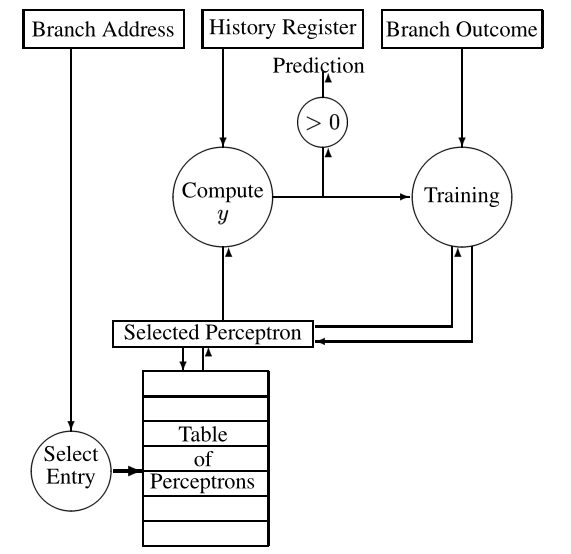
\includegraphics[scale = 0.4]{master thought.png}
\end{center}
In general, we need:
\begin{itemize}
  \item A \textbf{Perceptrons Table} to store all groups of weights respect to different hash value of branch addresses
  \item A \textbf{History Register} to store all informations (take as $1$/not take as $-1$) of different previous dynamic flow branches.
\end{itemize} 
Each time we get a branch instruction at decode stage:
\begin{itemize}
  \item First we hash the PC address, take the hash value as the index of \textbf{Perceptrons Table} and select out a group of weights.
  \item Second, we calculate the output $y$ of perceptron by using the weights $w_{i}$ and history branches value $x_{i}$ in \textbf{History Register}. $y=w_{0}+\sum_{i=1}^{n}x_{i}w_{i}$. The $w_{0}$ is a bias.
  \item If $y$ is negative, return a result of branch prediction untaken. If $y$ is non-negative, return a result of branch prediction taken.  
\end{itemize}
Each time we get the result of a branch at excute stage:
\begin{itemize}
  \item We calculate the $y_{out}$ which is used for training, if output $y$ is larger than thresold, $y_{out}$ is 1, if $y$ is less than negative threshold, $y_{out}$ is -1, otherwise, $y_{out}$ is 0.
  \item Compare $y_{out}$ with the result $t$ (1 as taken, -1 as not taken) of the corresponding branch, if they are same, the previous prediction is correct, while others are incorrect.
  \item If the previous prediction is correct
    \begin{itemize}
      \item Do nothing
    \end{itemize}
  \item If the previous prediction is not correct
    \begin{itemize}
      \item Update the corresponding(PC hash value index) perceptron weights in \textbf{Perceptron Table}, $w = w + t^Tx$
    \end{itemize}
  \item We update \textbf{History Register}
    \begin{itemize}
      \item We first find LRU index $i$ of \textbf{History Registor}
      \item We evit the $i$th register, replace it by the current branch and its result.
    \end{itemize}
\end{itemize}

\section{Code Implementation}
\textbf{BranchPredictor.h}
\begin{lstlisting}[language=c++]
class BranchPredictor
{
public:
  enum Strategy
  {
    ...
    PERCEPTRON /* Branch Perceptron */
  } strategy;
  ...
private:
  std::vector<std::vector<int8_t>> tableOfPerceptron;
  std::vector<std::vector<int8_t>> historyTable;
  uint32_t lastRefence = 0;   /* To maintian LRU of history branch */
  int32_t yOut = 0;
}
\end{lstlisting}
\textbf{BranchPredictor.c, BranchPredictor::predict()}
\begin{lstlisting}[language=c++]
bool BranchPredictor::predict(uint32_t pc, uint32_t insttype, 
    int64_t op1, int64_t op2, int64_t offset)
  {
    switch (this->strategy)
    {
    ...
    case PERCEPTRON:
    {
      uint32_t hashPC = (pc % (HARDWARE_BUDGET * 1024)); /* PC hash value */
      int32_t output = 0; /* initialize */
      for (int i = 0; i < HISTORY_LENGTH; i++)
      {
        output += this->tableOfPerceptron[hashPC][i]*this->historyTable[i][0];
      }
      /* add bias */
      output += this->tableOfPerceptron[hashPC][HISTORY_LENGTH];
      /* calculate y-out for training */
      if (output > THRESHOLD)
      {
        this->yOut = 1;
      }
      else if (output < -THRESHOLD)
      {
        this->yOut = -1;
      }
      else
      {
        this->yOut = 0;
      }
      /* result of prediction */
      if (output < 0)
      {
        return false;
      }
      else
      {
        return true;
      }
    }
    break;
    default:
      dbgprintf("Unknown Branch Perdiction Strategy!\n");
      break;
    }
    return false;
  }
\end{lstlisting}
\textbf{BranchPredictor.c, BranchPredictor::update()}
\begin{lstlisting}[language=c++]
void BranchPredictor::update(uint32_t pc, bool branch)
{
  ...
  if (branch)
  {
    this->lastRefence++;  /* Maintain LRU refence */
    if (this->strategy == PERCEPTRON)
    {
      if (this->yOut != 1)
      { /* If yout != result, update weights */
        uint32_t hashPC = (pc % (HARDWARE_BUDGET * 1024));
        for (int i = 0; i < HISTORY_LENGTH; i++)
        {
          this->tableOfPerceptron[hashPC][i] += this->historyTable[i][0];
        }
        this->tableOfPerceptron[hashPC][HISTORY_LENGTH]++;
      }
    }
    else
    { /* Other predict mode keep same */
      if (state == STRONG_NOT_TAKEN)
      {
        this->predbuf[id] = WEAK_NOT_TAKEN;
      }
      else if (state == WEAK_NOT_TAKEN)
      {
        this->predbuf[id] = WEAK_TAKEN;
      }
      else if (state == WEAK_TAKEN)
      {
        this->predbuf[id] = STRONG_TAKEN;
      } // do nothing if STRONG_TAKEN
    }

    int8_t index = findReplaceIndexOfHistoryTable();  /* Find the LRU place */
    this->historyTable[index][0] = 1;            /* Update result of branch */
    this->historyTable[index][1] = this->lastRefence; /* Update LRU refence */
  }
  else
  {
    this->lastRefence++;
    if (this->strategy == PERCEPTRON)
    {
      if (this->yOut != -1)
      { /* If yout != result, update weights */
        uint32_t hashPC = (pc % (HARDWARE_BUDGET * 1024));
        for (int i = 0; i < HISTORY_LENGTH; i++)
        {
          this->tableOfPerceptron[hashPC][i] -= this->historyTable[i][0];
        }
        this->tableOfPerceptron[hashPC][HISTORY_LENGTH]--;
      }
    }
    else
    {
      /* Other predict mode keep same */
      if (state == STRONG_TAKEN)
      {
        this->predbuf[id] = WEAK_TAKEN;
      }
      else if (state == WEAK_TAKEN)
      {
        this->predbuf[id] = WEAK_NOT_TAKEN;
      }
      else if (state == WEAK_NOT_TAKEN)
      {
        this->predbuf[id] = STRONG_NOT_TAKEN;
      } // do noting if STRONG_NOT_TAKEN
    }

    int8_t index = findReplaceIndexOfHistoryTable();  /* Find the LRU place */
    this->historyTable[index][0] = -1;           /* Update result of branch */
    this->historyTable[index][1] = this->lastRefence; /* Update LRU refence */
  }
}
\end{lstlisting}

\textbf{BranchPredictor.c, BranchPredictor::findReplaceIndexOfHistoryTable()}
\begin{lstlisting}[language=c++]
/* Function to find replace branch in history table */ 
int8_t BranchPredictor::findReplaceIndexOfHistoryTable(void)
{
  int32_t minTmp = this->historyTable[0][1];
  int8_t index = 0;
  for (int i = 0; i < HISTORY_LENGTH; i++)
  {
    if (this->historyTable[i][1] < minTmp)
    {
      minTmp = this->historyTable[i][1];
      index = i;
    }
  }
  return index;
}
\end{lstlisting}
While some other basic implementation I'll not list here, such as, modify functions to parse \textbf{pc} in class \textbf{BranchPredictor}, initialize vectors stated in \textbf{BranchPredictor.h}, etc.. They are too simple and naive to list here.

\section{Basic Implementation Correctness and Performance}
\subsection{Correctness}
I simply run three test, \textbf{quicksort.c, ackermann.c, matrixmulti.c}, here is three result\\
\begin{center}
  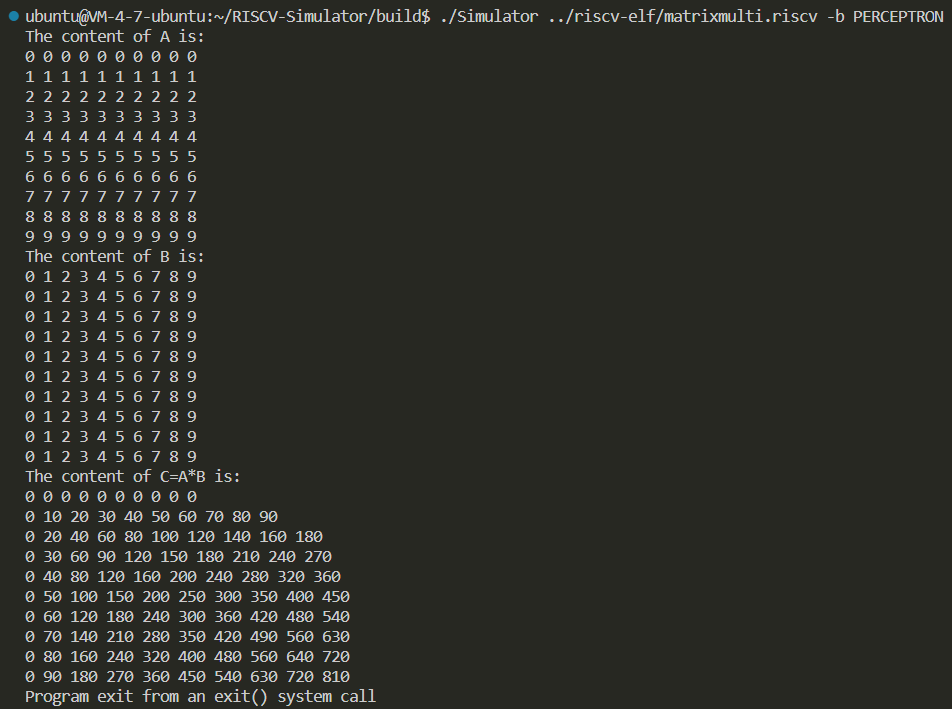
\includegraphics[scale = 0.4]{correctness matrix.png}\\
  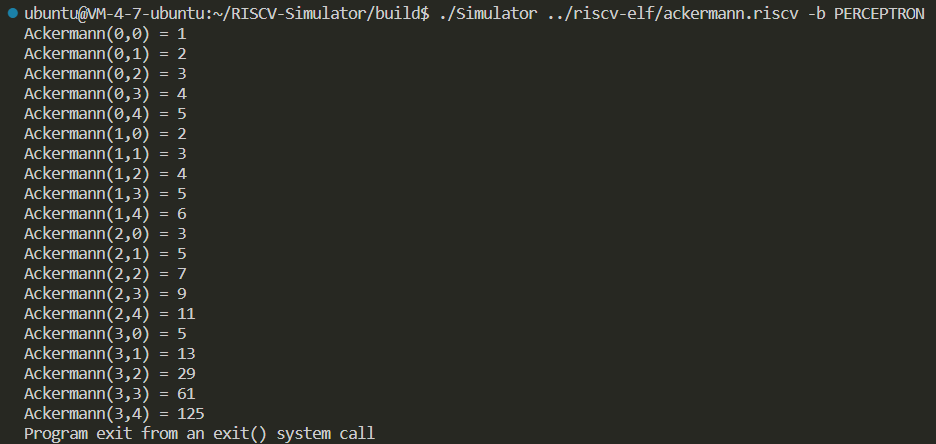
\includegraphics[scale = 0.4]{correctness acker.png}\\
  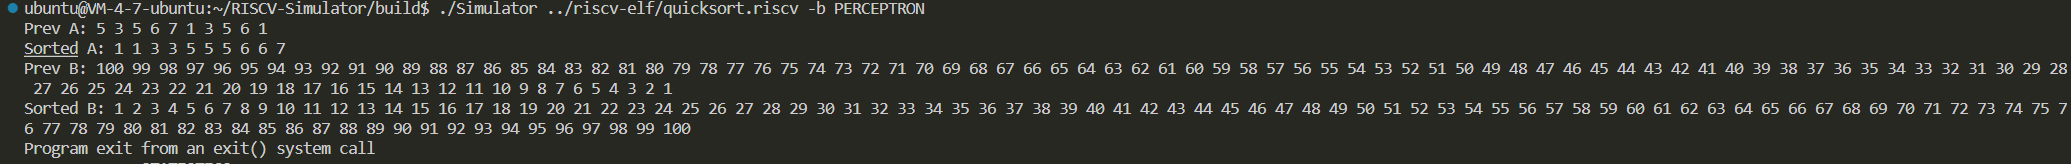
\includegraphics[scale = 0.25]{correctness quick.png}
\end{center}
We can clear see that three programs all excuted correctly.
\subsection{Performance}
I still use these three programs, \textbf{quicksort.c, ackermann.c, matrixmulti.c}, I apply all \textbf{Always Taken, Always Not Taken, Back Taken Forward Not Taken, Branch Prediction Buffer, Dynamic Branch Prediction with Perceptron} prediction policy and thus get a table. In this table, horizontal axis is the policies, the vertical axis is three test programs, and the remaining is the correct prediction percent.
\begin{center}
  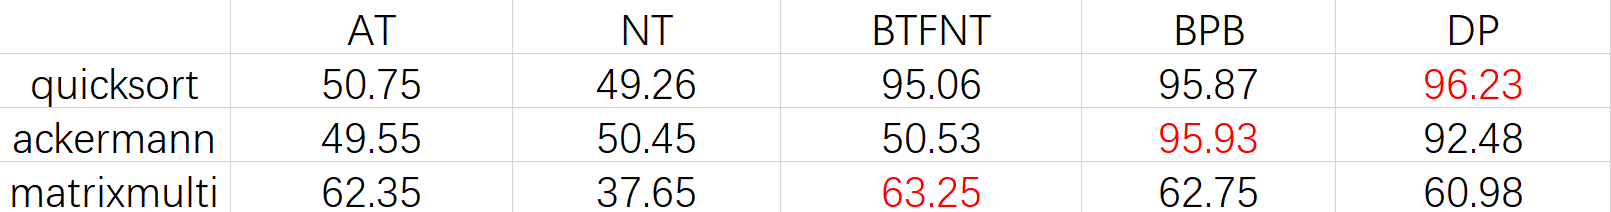
\includegraphics[scale = 0.3]{naive result.png}\\
\end{center}
The highlighed block is the highest correct prediciton percent of each program among five policies. \\
We find that, \textbf{Dynamic Branch Prediction with Perceptron} perform best in \textbf{quicksort.c}, but perform worse in \textbf{ackermann.c} with $3.45\%$ distance, in \textbf{matrixmulti.c} with $2.27\%$ distance.

\section{Analysis and Improvement}
\subsection{Why all perform bad in \textbf{matrixmulti.c}}
As we look into the codes, we can find that \textbf{matrixmulti.c} has many large nested(three maximum) loop, the deepest loop's code only excute $10$ times each enueration, which means many dynamic flow branch do not have a proper pattern to predict or learn. This problem cannot solved by only change the parameter of perceptron, multilayer perceptron might learn this kind of pattern well, but it will be a large overhead on hardware.
\subsection{How to prove naive single layor perceptron}
As I noticed, if the prediction is wrong, \textbf{Dynamic Branch Prediction with Perceptron} policy will training the weights by adding an inverse gradient step. Thus, this policy often fails when there come a new branch in dynamic logical flow. Also, it always fails in the next few prediction because each time the weights only change by only $1$ step. My thinking is that, if I detect that the previous branch is same with what I current excute, and my prediction is same with the previous branch result, I will change the weights by another gradient step.\\
Also, I noticed that each time we evit a LRU dynamic flow branch out of \textbf{History Register}, the corresponding weights in all entries of \textbf{Perceptrons Table} should be changed, too. Now, these invalid weights just keep the same, but it will cause problem if the new branch result is different with the LRU branch result, which means the weights should not be inherited. So I add more steps, if two branches noted before are same in result, I just keep the weights unchanged, if they are different, I will change the weights all to $1$ is the new branch is result in taken, $-1$ otherwise.\\
Here is the code.\\
\textbf{BranchPredictor.h}
\begin{lstlisting}[language=c++]
  class BranchPredictor
  {
    ...
  private:
    ...
    uint32_t lastPc = 0; /* To store previous branch PC */
    bool lastRes = 0;    /* To store previous branch result */
    ...
  }
\end{lstlisting}
\textbf{BranchPredictor.c, BranchPredictor::update()}
\begin{lstlisting}[language=c++]
void BranchPredictor::update(uint32_t pc, bool branch)
{
  ...
  if (branch)
  {
    ...
    if (this->strategy == PERCEPTRON)
    {
      ...
      if (pc == this->lastPc && branch == this->lastRes)
      { /* If all same, give additional training */
        this->tableOfPerceptron[hashPC][HISTORY_LENGTH] += 1;
      }
    }
    ...
    this->lastPc = pc;
    this->lastRes = branch;
  }
  else
  {
    ...
    if (this->strategy == PERCEPTRON)
    {
      ...
      if (pc == this->lastPc && branch == this->lastRes)
      { /* If all same, give additional training */
        this->tableOfPerceptron[hashPC][HISTORY_LENGTH] -= 1;
      }
    }
    ...
    this->lastPc = pc;
    this->lastRes = branch;
  }
}
\end{lstlisting}
Here is the result, which highlighed in purpose.
\begin{center}
  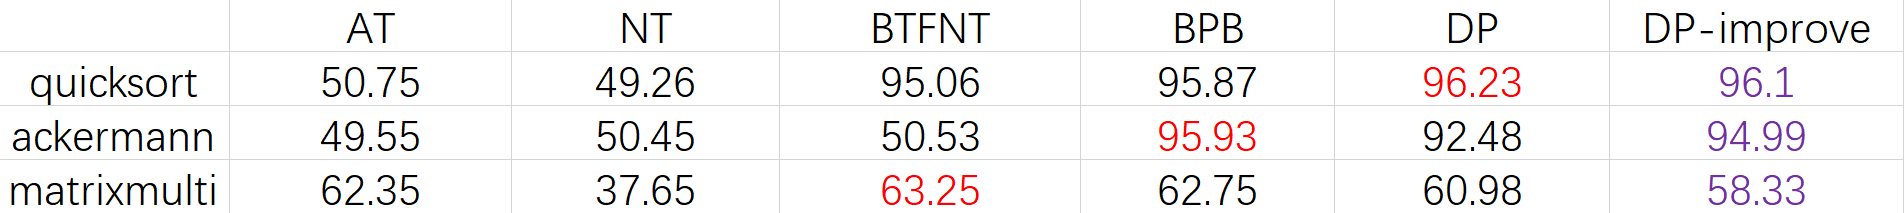
\includegraphics[scale = 0.25]{prove result.png}\\
\end{center}
We can see that, this implementation sacrificed only $0.13\%$ percent of \textbf{quicksort.c} branch prediction correct rate to gain $2.41\%$ percent of \textbf{ackermann.c} branch prediction correct rate. But the \textbf{matrixmulti.c} branch prediction correct rate is still a big problem.
\end{document}
